% !TeX TXS-program:compile = txs:///lualatex

\documentclass[french,11pt,a4paper]{article}
%\usepackage[utf8]{inputenc}
%\usepackage[T1]{fontenc}
\usepackage{amsmath,amssymb}
\usepackage{fontspec}
\setmonofont[Scale=MatchLowercase]{Inconsolatazi4}
\usepackage{tkz-bernoulli}
\usepackage{nicefrac}
\usepackage{enumitem}
\usepackage{codehigh}
\usepackage{multicol}
\usepackage{tabularray}
\usepackage{lipsum}
\usepackage{fancyvrb}
\usepackage{fancyhdr}
\usepackage{fontawesome5}
\fancyhf{}
\renewcommand{\headrulewidth}{0pt}
%\rhead{\sffamily\small\affloetalab[Legende]}
\lfoot{\sffamily\small [tkz-bernoulli]}
\cfoot{\sffamily\small - \thepage{} -}
\rfoot{\hyperlink{matoc}{\small\faArrowAltCircleUp[regular]}}
\usepackage{hologo}
\providecommand\tikzlogo{Ti\textit{k}Z}
\providecommand\TeXLive{\TeX{}Live\xspace}
\providecommand\PSTricks{\textsf{PSTricks}\xspace}
\let\pstricks\PSTricks
\let\TikZ\tikzlogo

\usepackage{hyperref}
\urlstyle{same}
\hypersetup{pdfborder=0 0 0}
\usepackage[margin=1.5cm]{geometry}
\setlength{\parindent}{0pt}
\def\TPversion{0.1.0}
\def\TPdate{9 septembre 2023}
\usepackage{tcolorbox}
\tcbuselibrary{skins,hooks}
\usepackage{soul}
\sethlcolor{lightgray!25}
\NewDocumentCommand\MontreCode{ m }{%
	\hl{\vphantom{\texttt{pf}}\texttt{#1}}%
}
\usepackage{siunitx}
\sisetup{locale=FR}
\usepackage{babel}

\begin{document}

\pagestyle{fancy}

\thispagestyle{empty}

\begin{center}
	\begin{minipage}{0.88\linewidth}
	\begin{tcolorbox}[colframe=yellow,colback=yellow!15]
		\begin{center}
			\begin{tabular}{c}
				{\Huge \texttt{tkz-bernoulli}}\\
				\\
				{\LARGE Présenter, grâce à \MontreCode{tikz},} \\
				{\LARGE des arbres de Bernoulli.} \\
				\\
				{\LARGE $\rhd$ Commandes [fr] ou [en] $\lhd$} \\
				\\
				{\small \texttt{Version \TPversion{} -- \TPdate}}
		\end{tabular}
		\end{center}
	\end{tcolorbox}
\end{minipage}
\end{center}

\begin{center}
	\begin{tabular}{c}
		\texttt{Cédric Pierquet}\\
		{\ttfamily c pierquet -- at -- outlook . fr}\\
		\texttt{\url{https://github.com/cpierquet/tkz-bernoulli}} \\
	\end{tabular}
\end{center}

\hrule

\vfill

Présenter, avec personnalisations possibles, un arbre de Bernoulli.

\vfill

\begin{tcolorbox}[colframe=lightgray,colback=white]
\MontreCode{\textbackslash tkzSchemBernoulli*}

\hfill\tkzSchemBernoulli*\hfill~
\end{tcolorbox}

\vspace*{5mm}

\begin{tcolorbox}[colframe=lightgray,colback=white]
\MontreCode{\textbackslash tkzSchemBernoulli*}

\phantom{\texttt{~~~~}}\MontreCode{[N=2,EspNiv=3,EspFeuil=1.25,NoticeProbas=\{\textbackslash num{0.75}/\textbackslash num\{0.25\}\},Evts=\{\$E\$/\$\textbackslash overline\{E\}\$\}]}

\tikzstyle{BernProbaS} = [text=violet,fill=white,sloped,midway,font=\scriptsize]
\tikzstyle{BernProbaE} = [text=red,fill=white,sloped,midway,font=\scriptsize]
\tikzstyle{BernBranche} = [semithick,blue,->]
\hfill\tkzSchemBernoulli*[N=2,EspNiv=3,EspFeuil=1.25,Notice,Racine=false,Probas={\num{0.75}/\num{0.25}},Evts={$E$/$\overline{E}$}]\hfill~
\tkzSchemBernStyleDefaut
\end{tcolorbox}

\vfill~

\pagebreak

\phantomsection

\hypertarget{matoc}{}

\tableofcontents

\vspace*{5mm}

\hrule

\vspace*{5mm}

\section{Le package tkz-bernoulli}

\subsection{Introduction}

L'idée du package \MontreCode{tkz-bernoulli} est de proposer des commandes pour représenter un schéma de Bernoulli, dans le cadre d'une loi binomiale par exemple, avec la possibilité de :

\begin{itemize}
	\item personnaliser les dimensions et styles ;
	\item rajouter des éléments a posteriori, grâce aux nœuds créés.
\end{itemize}

\subsection{Chargement}

Le package se charge dans le préambule, via \MontreCode{\textbackslash usepackage\{tkz-bernoulli\}}.

Les seuls packages chargés sont :

\begin{itemize}
	\item \MontreCode{xstring}, \MontreCode{pgffor} et \MontreCode{simplekv} ;
	\item \MontreCode{xintexpr} et \MontreCode{xintbinhex} ;
	\item \MontreCode{tikz} avec la librairie \MontreCode{calc}.
\end{itemize}

\begin{codehigh}[language=latex/latex2,style/main=cyan!10,style/code=cyan!10]
\usepackage{tkz-bernoulli}
\end{codehigh}

{\small\faAngleDoubleRight}~\MontreCode{tkz-bernoulli} est compatible avec les compilations usuelles en \textsf{latex}, \textsf{pdflatex}, \textsf{lualatex} ou \textsf{xelatex}.

\subsection{Commandes disponibles}

Les commandes proposées par le package \MontreCode{tkz-bernoulli} sont :

\begin{codehigh}[language=latex/latex2,style/main=cyan!10,style/code=cyan!10]
%commande à insérer dans un environnement tikzpicture, pour rajouts éventuels
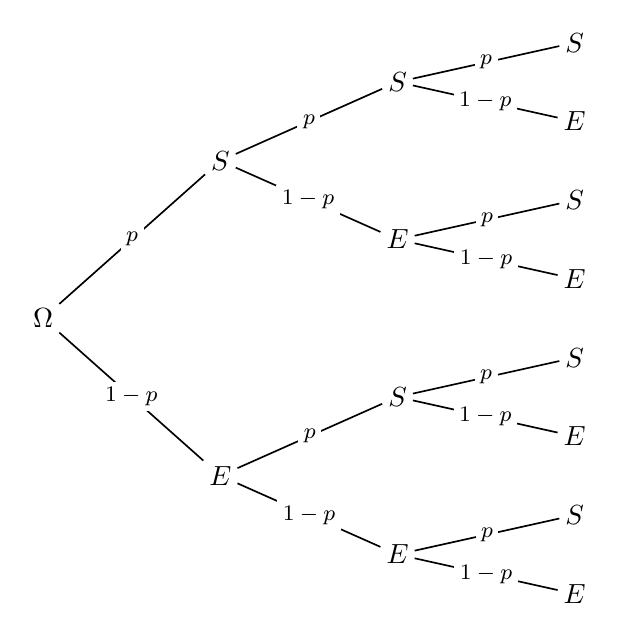
\begin{tikzpicture}
    \tkzSchemBernoulli
\end{tikzpicture}
\end{codehigh}

\begin{codehigh}[language=latex/latex2,style/main=cyan!10,style/code=cyan!10]
%commande autonome
\tkzSchemBernoulli*
\end{codehigh}

\subsection{Styles par défaut}

Le package propose des styles prédéfinis, pour :

\begin{itemize}
	\item la racine et  les nœuds ;
	\item les branches ;
	\item les probabilités.
\end{itemize}

Pour modifier, en \textit{profondeur}, le style de l'arbre, il suffira de redéfinir les styles suivants (une commande est disponible pour remettre tous les styles par défaut) :

\begin{codehigh}[language=latex/latex2,style/main=cyan!10,style/code=cyan!10]
%style par défaut des branches
\tikzstyle{BernBranche} = [semithick]

%style par défaut du label de la racine, si affichée
\tikzstyle{BernRacine} = [inner sep=2pt]

%styles par défaut des noeuds relatifs à Succès/Échec
\tikzstyle{BernNoeudS} = [inner sep=2pt]
\tikzstyle{BernNoeudE} = [inner sep=2pt]

%styles par défaut des probas relatives à Succès/Échec
\tikzstyle{BernProbaS} = [fill=white,midway,font=\footnotesize,inner sep=1.5pt]
\tikzstyle{BernProbaE} = [fill=white,midway,font=\footnotesize,inner sep=1.5pt]

%style par défaut des valeurs prises par la v.a.
\tikzstyle{BernNotice} = [inner sep=2pt,text=teal,right=1em]
\end{codehigh}

\begin{codehigh}[language=latex/latex2,style/main=cyan!10,style/code=cyan!10]
%commande de remise des styles par défaut
\tkzSchemBernStyleDefaut
\end{codehigh}

\section{Les commandes}

\subsection{Commande à insérer dans un environnement tikzpicture}

La commande dédiée pour insertion dans un environnement \textsf{tikzpicture} est \MontreCode{\textbackslash tkzSchemBernoulli} :

\begin{codehigh}[language=latex/latex2,style/main=cyan!10,style/code=cyan!10]
%commande à insérer dans un environnement tikzpicture, pour rajouts éventuels
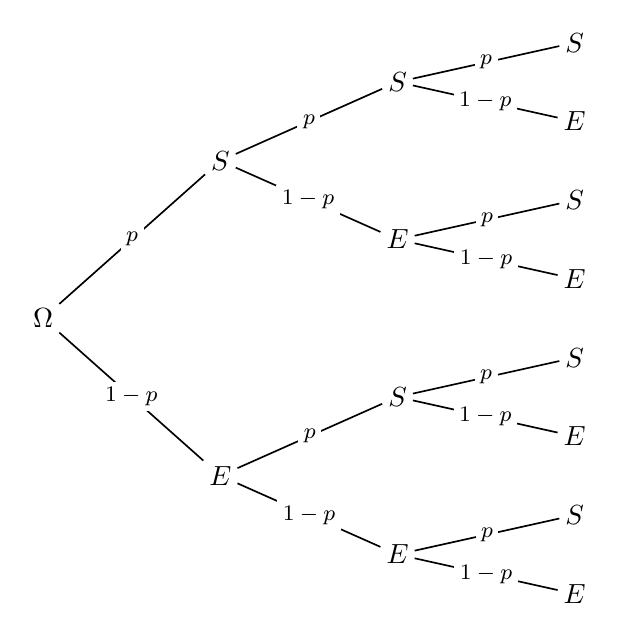
\begin{tikzpicture}
    \tkzSchemBernoulli[clés]
\end{tikzpicture}
\end{codehigh}

Concernant cette commande :

\begin{itemize}
	\item les clés disponibles sont :
	\begin{itemize}
		\item \MontreCode{EspNiv} := espace horizontal entre les niveaux (\MontreCode{2.25} par défaut) ;
		\item \MontreCode{EspFeuil} := espace vertical entre les éléments du dernier niveau (\MontreCode{1} par défaut) ;
		\item \MontreCode{Evts} := nom des évènements Succès/Échec (\MontreCode{\$S\$/\$E\$} par défaut) ;
		\item \MontreCode{Probas} := probabilités (\MontreCode{\$p\$/\$1-p\$} par défaut) ;
		\item \MontreCode{AffProbas} := booléen pour afficher les probabilités (\MontreCode{true} par défaut) ;
		\item \MontreCode{Racine} := nom qui apparaît pour la racine(\MontreCode{\$\textbackslash Omega\$} par défaut, ou \MontreCode{false} pour désactiver) ;
		\item \MontreCode{Aide} := booléen pour afficher les noms des nœuds créés (\MontreCode{false} par défaut) ;
		\item \MontreCode{Notice} := booléen pour afficher les valeurs prises par la v.a. (\MontreCode{false} par défaut) ;
		\item \MontreCode{Var} := nom de la v.a. pour la notice (\MontreCode{X} par défaut) ;
		\item \MontreCode{N} := paramètre $n$ du schéma de Bernoulli (\MontreCode{3} par défaut).
	\end{itemize}
\end{itemize}

\begin{demohigh}[language=latex/latex2,style/main=cyan!10,style/code=cyan!10]
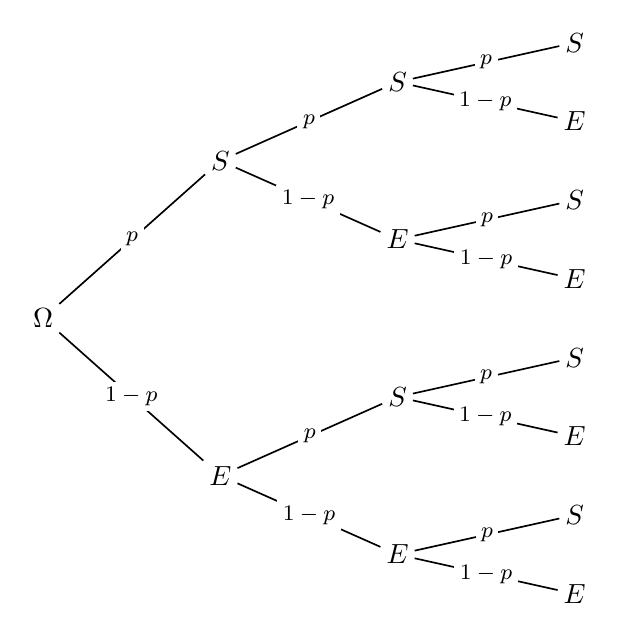
\begin{tikzpicture}
    \tkzSchemBernoulli
\end{tikzpicture}
\end{demohigh}

\begin{demohigh}[language=latex/latex2,style/main=cyan!10,style/code=cyan!10]
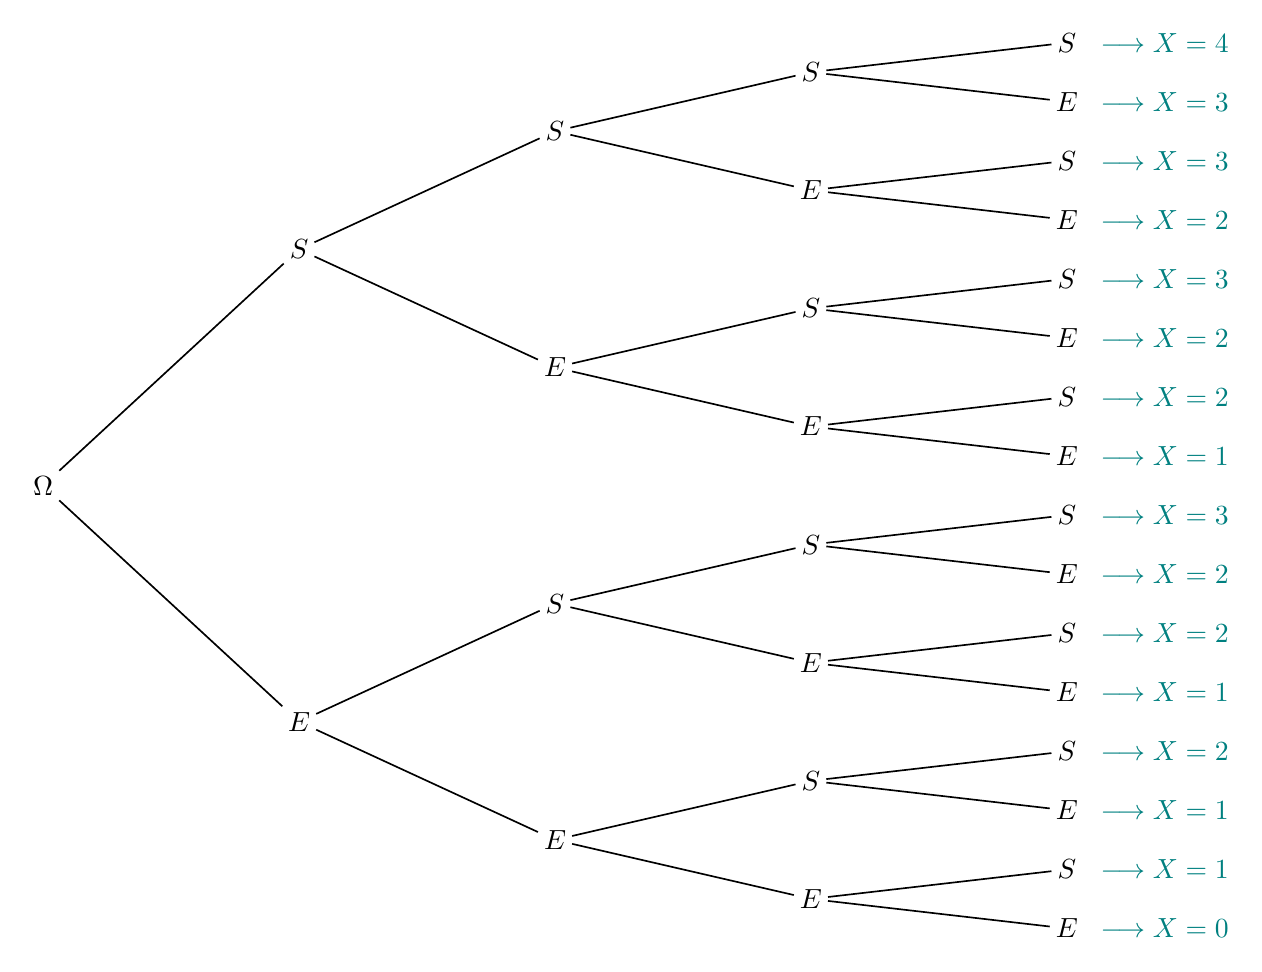
\begin{tikzpicture}
    \tkzSchemBernoulli[Notice,AffProbas=false,EspNiv=3.25,EspFeuil=0.75,N=4]
\end{tikzpicture}
\end{demohigh}

\begin{demohigh}[language=latex/latex2,style/main=cyan!10,style/code=cyan!10]
%\usepackage{nicefrac}
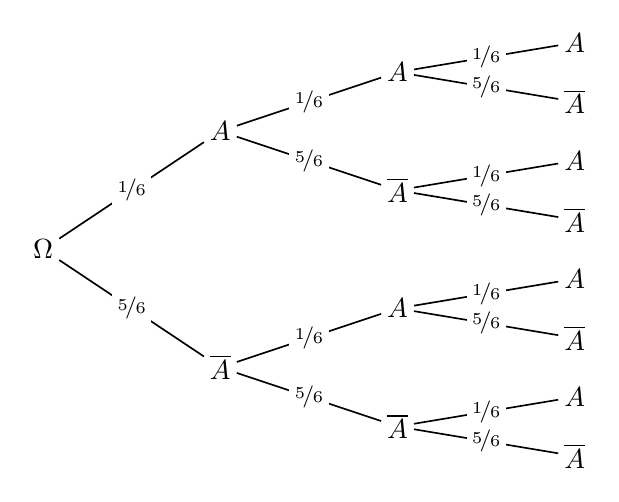
\begin{tikzpicture}
    \tkzSchemBernoulli[%
        Evts={$A$/$\overline{A}$},%
        EspFeuil=0.75,%
        Probas={$\nicefrac{1}{6}$/$\nicefrac{5}{6}$}]
\end{tikzpicture}
\end{demohigh}

\subsection{Commande autonome}

La commande dédiée pour insertion autonome est \MontreCode{\textbackslash tkzSchemBernoulli*} :

\begin{codehigh}[language=latex/latex2,style/main=cyan!10,style/code=cyan!10]
%commande autonome
\tkzSchemBernoulli*[clés]<options tikz>
\end{codehigh}

Concernant cette commande :

\begin{itemize}
	\item l'environnement \textsf{tikzpicture} est automatiquement créé ;
	\item les \textsf{clés} sont les mêmes que pour la commande non étoilée ;
	\item des \MontreCode{<options tikz>}, optionnels, peuvent être passées à l'environnement \textsf{tikzpicture}.
\end{itemize}

\begin{demohigh}[language=latex/latex2,style/main=cyan!10,style/code=cyan!10]
\tkzSchemBernoulli*
\end{demohigh}

\begin{demohigh}[language=latex/latex2,style/main=cyan!10,style/code=cyan!10]
\tkzSchemBernoulli*[Notice,AffProbas=false,EspNiv=3.25,EspFeuil=0.75,N=4,Aide]
\end{demohigh}

\begin{demohigh}[language=latex/latex2,style/main=cyan!10,style/code=cyan!10]
%\usepackage{nicefrac}
\tkzSchemBernoulli*[%
    N=6,EspFeuil=0.35,Notice,%
    Probas={$\nicefrac{1}{6}$/$\nicefrac{5}{6}$}]
    <scale=0.75,every node/.style={scale=0.5}>
\end{demohigh}

\pagebreak

\subsection{Mofication avancée des styles}

Les \textsf{clés} relatives aux commandes précédentes permettent de modifier l'aspect \textit{global} de l'arbre, mais les styles particuliers des éléments peuvent également être modifiés, comme indiqué au début de cette documentation.

\begin{demohigh}[language=latex/latex2,style/main=cyan!10,style/code=cyan!10]
\tikzstyle{BernBranche} = [thick,red,->]
\tikzstyle{BernRacine}  = []
\tikzstyle{BernNoeudS}  = [draw,rectangle,inner sep=1.5pt]
\tikzstyle{BernNoeudE}  = [draw,rectangle,inner sep=1.5pt]
\tikzstyle{BernProbaS}  = [text=teal,midway,fill=cyan!5,inner sep=1.5pt]
\tikzstyle{BernProbaE}  = [text=orange,midway,fill=purple!5,inner sep=1.5pt]
\tkzSchemBernoulli*
\end{demohigh}

\pagebreak

\section{English commands}

\subsection{Introduction}

There's also english versions of the commands and keys :

\begin{codehigh}[language=latex/latex2,style/main=cyan!10,style/code=cyan!10]
%command in an environment tikzpicture
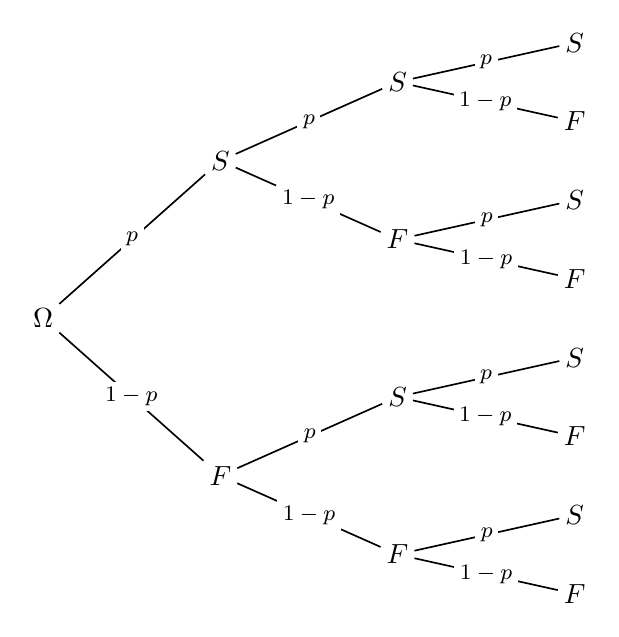
\begin{tikzpicture}
    \tkzBernoulliTree[keys]
\end{tikzpicture}
\end{codehigh}

\begin{codehigh}[language=latex/latex2,style/main=cyan!10,style/code=cyan!10]
%stand-alone command
\tkzBernoulliTree*[keys]<tikz options>
\end{codehigh}

Default styles are given by :

\begin{codehigh}[language=latex/latex2,style/main=cyan!10,style/code=cyan!10]
%style for edges
\tikzstyle{BernEdge} = [semithick]

%style for root (if displayed)
\tikzstyle{BernRoot} = [inner sep=2pt]

%styles for nodes Success/Failure
\tikzstyle{BernNodeS} = [inner sep=2pt]
\tikzstyle{BernNodeF} = [inner sep=2pt]

%styles for probas Success/Failure
\tikzstyle{BernProbS} = [fill=white,midway,font=\footnotesize,inner sep=2pt]
\tikzstyle{BernProbF} = [fill=white,midway,font=\footnotesize,inner sep=2pt]

%style for values taken by X
\tikzstyle{BernGuide} = [inner sep=2pt,text=teal,right=1em]
\end{codehigh}

\begin{codehigh}[language=latex/latex2,style/main=cyan!10,style/code=cyan!10]
%command to restore default styles
\tkzBernTreeStyleDefault
\end{codehigh}

\subsection{Examples}

\begin{demohigh}[language=latex/latex2,style/main=cyan!10,style/code=cyan!10]
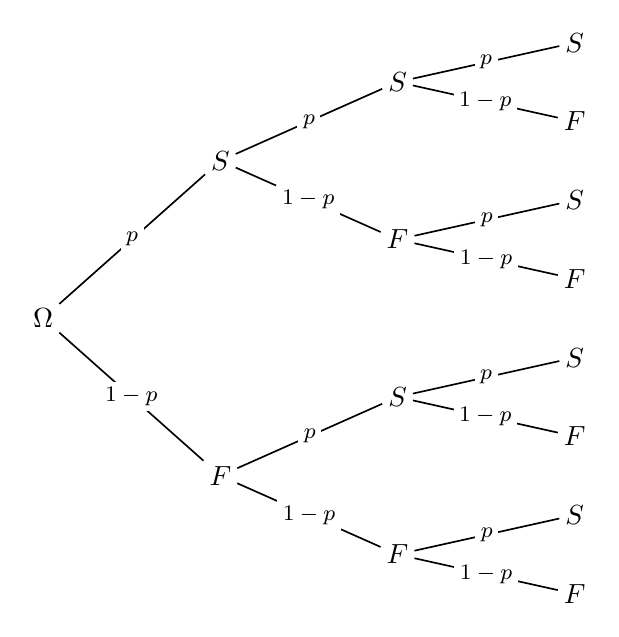
\begin{tikzpicture}
    \tkzBernoulliTree
\end{tikzpicture}
\end{demohigh}

\begin{demohigh}[language=latex/latex2,style/main=cyan!10,style/code=cyan!10]
\tkzBernoulliTree*[Help,ShowProbs=false,LevelSep=3.25,NodeSep=0.75,N=4,Guide,var=Z]
\end{demohigh}

\begin{demohigh}[language=latex/latex2,style/main=cyan!10,style/code=cyan!10]
%\usepackage{nicefrac}
\tikzstyle{BernEdge}  = [thick,red,->]
\tikzstyle{BernRoot}  = []
\tikzstyle{BernNodeS} = [draw,rectangle,fill=yellow,inner sep=1.5pt]
\tikzstyle{BernNodeF} = [draw,rectangle,fill=orange,inner sep=1.5pt]
\tikzstyle{BernProbS} = [text=teal,midway,fill=cyan!5,inner sep=1.5pt]
\tikzstyle{BernProbF} = [text=orange,midway,fill=purple!5,inner sep=1.5pt]
\tikzstyle{BernGuide} = [draw,rectangle,inner sep=2pt,text=green,right=2em]
\tkzBernoulliTree*[%
    Events={$A$/$\overline{A}$},%
    NodeSep=0.75,Guide,%
    Probs={$\nicefrac{1}{6}$/$\nicefrac{5}{6}$}]
\end{demohigh}

\end{document}